\documentclass{article}

\usepackage{times}
\usepackage{amssymb, amsmath, amsthm}
\usepackage[margin=.5in]{geometry}
\usepackage{graphicx}
\usepackage[linewidth=1pt]{mdframed}
\usepackage{bm}

\usepackage{import}
\usepackage{xifthen}
\usepackage{pdfpages}
\usepackage{transparent}
\usepackage{listings}

\newcommand{\incfig}[1]{%
    \def\svgwidth{\columnwidth}
    \import{./figures/}{#1.pdf_tex}
}

\newtheorem{theorem}{Theorem}[section]
\newtheorem{lemma}{Lemma}[section]
\newtheorem*{remark}{Remark}
\theoremstyle{definition}
\newtheorem{definition}{Definition}[section]

\begin{document}
\title{Machine Learning and Data Mining -- Homework 2}
\author{Philip Warton}
\date{\today}
\maketitle

\section*{Section 1}
    \subsection*{Q1}
Assume that we choose $\bm w$ such that the likelihood is maximal. Then, equivalently,
the natural log of the likelihood is also maximal. So we write that,
\begin{align*}
    \ln(\mathcal{L}) &= \ln\left(\prod P(y_i \ | \ x_i, \bm w)\right) \\
    &= \sum \left(
        \ln P(y_i \ | \ x_i, \bm w)
    \right) \\
    &= \sum \left(
        \ln \left(
            \frac{1}{2b}e^{-|y_i-\bm w^T x_i|/b}
        \right)
    \right) \\
    &= \sum(\ln \frac{1}{2b}) + \sum\left(
        \ln e^{|y_i - \bm w^T x_i|/b}
    \right)\\
    &= N\ln\frac{1}{2b} - \frac{N}{b} \sum |y_i - \bm w^T x_i|
\end{align*}
Since the first term is independent of $\bm w$ it is not relevant to what vector $\bm w$ maximizes this value.
So since the second term is negative, the likelihood is maximized when this term is minimized. Clearly,
this term is proportional to the sum of absolute errors, and the statement is proven.
    \subsection*{Q2}
Suppose we have a dataset as given by the problem. We now compute recall and precision.
\begin{center}
    \begin{tabular}{l|llllll}
              & $t=0$         & $t=0.2$        & $t=0.4$        & $t=0.6$       & $t=0.8$       & $t=1$         \\
\hline
    TP        & 8             & 8              & 6              & 6             & 4             & 0             \\
    FN        & 0             & 0              & 2              & 2             & 4             & 8             \\
    FP        & 8             & 6              & 3              & 1             & 1             & 0             \\
    Recall    & 1             & 1              & $3/4$  & $3/4$ & $1/2$ & $0$ \\
    Precision & $1/2$ & $4/7$ & $2/3$ & $6/7$ & $4/5$ & $UND$            
    \end{tabular}
\end{center}
\section*{Section 2}
    \subsection*{Q3}
\begin{lstlisting}[language=python]
def logistic(z):
    logit_z = 1 / (1 + np.exp(-1 * z))
    return logit_z
\end{lstlisting}
\begin{lstlisting}[language=python]
def calculateNegativeLogLikelihood(X, y, w):
    small_constant = 0.000000001
    nll = (-1) * np.sum(
        (np.log(logistic(w.T @ X.T) + small_constant) @ y) + 
        ((np.log(1 - logistic(w.T @ X.T) + small_constant)) @ (1 - y))
    )
    return nll
    \end{lstlisting}
    \subsection*{Q4}
\begin{lstlisting}[language=python]
def trainLogistic(X, y, max_iters=max_iters, step_size=step_size):
    w = np.zeros((X.shape[1], 1))
    losses = [calculateNegativeLogLikelihood(X, y, w)]
    for i in range(max_iters):
        w_grad = X.T @ (logistic(X @ w) - y)
        assert(w_grad.shape == (X.shape[1], 1))
        w = w - step_size * w_grad
        losses.append(calculateNegativeLogLikelihood(X, y, w))
    return w, losses
\end{lstlisting}
    \subsection*{Q5}
    \begin{lstlisting}[language=python]
def dummyAugment(X):
    n = len(X)
    one_col = np.ones((n, 1))
    X_augmented = np.hstack((one_col, X))
    return X_augmented
    \end{lstlisting}
    \subsection*{Q6}
For each step size we have the following:\\\\

\begin{mdframed}[]
    \fbox{$n = 1$}
    \begin{verbatim}
Running cross-fold validation for bias case:
2-fold Cross Val Accuracy -- Mean (stdev): 94.64% (2.361%)
3-fold Cross Val Accuracy -- Mean (stdev): 96.78% (0.01962%)
4-fold Cross Val Accuracy -- Mean (stdev): 96.15% (1.95%)
5-fold Cross Val Accuracy -- Mean (stdev): 95.69% (1.437%)
10-fold Cross Val Accuracy -- Mean (stdev): 96.13% (2.987%)
20-fold Cross Val Accuracy -- Mean (stdev): 95.62% (4.264%)
50-fold Cross Val Accuracy -- Mean (stdev): 95.53% (7.089%)
    \end{verbatim}
    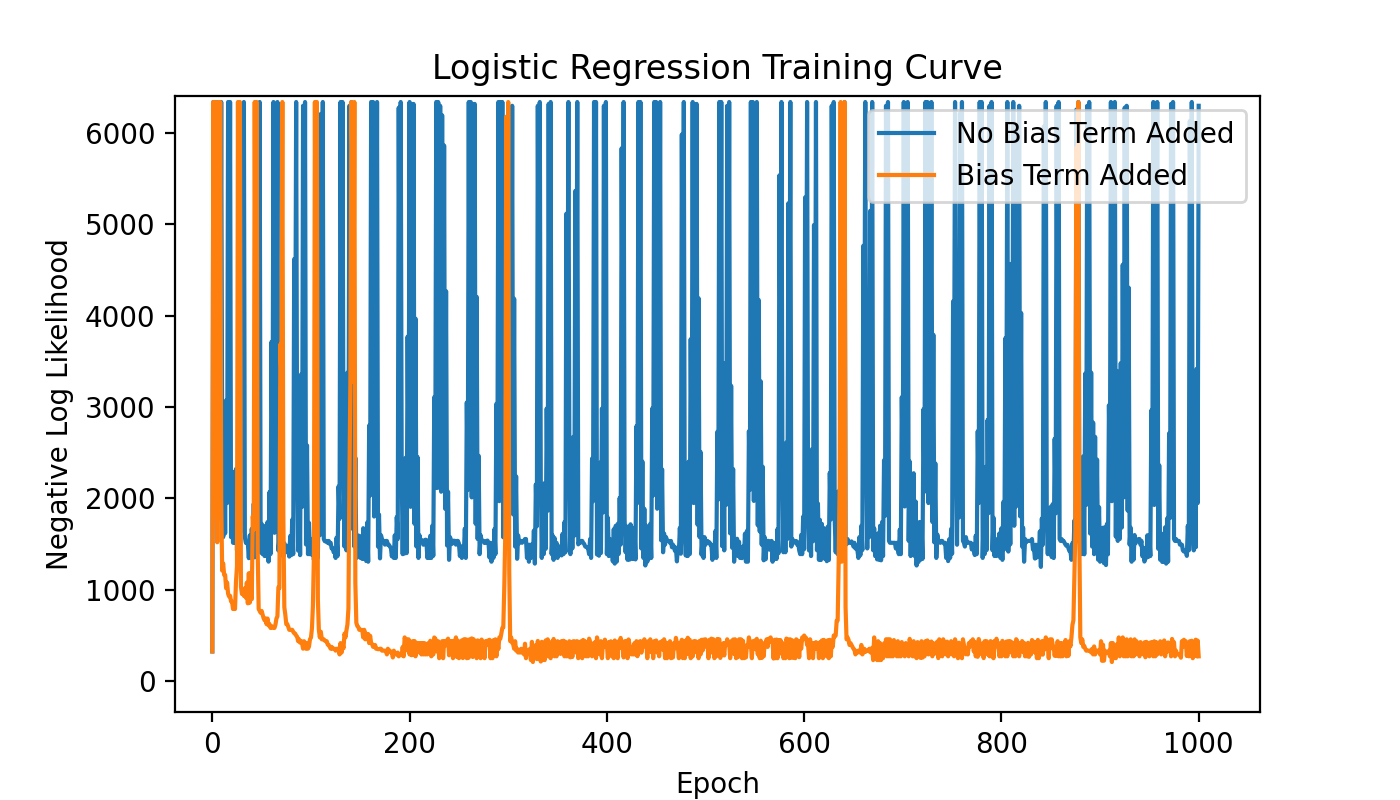
\includegraphics[scale=0.75]{figures/step_size_1.png}
\end{mdframed}

\begin{mdframed}[]
    \fbox{$n = 0.1$}
    \begin{verbatim}
Running cross-fold validation for bias case:
2-fold Cross Val Accuracy -- Mean (stdev): 93.56% (1.288%)
3-fold Cross Val Accuracy -- Mean (stdev): 92.69% (2.648%)
4-fold Cross Val Accuracy -- Mean (stdev): 95.51% (2.585%)
5-fold Cross Val Accuracy -- Mean (stdev): 96.75% (2.41%)
10-fold Cross Val Accuracy -- Mean (stdev): 94.83% (3.069%)
20-fold Cross Val Accuracy -- Mean (stdev): 95.83% (4.37%)
50-fold Cross Val Accuracy -- Mean (stdev): 95.53% (7.383%)  
    \end{verbatim}
    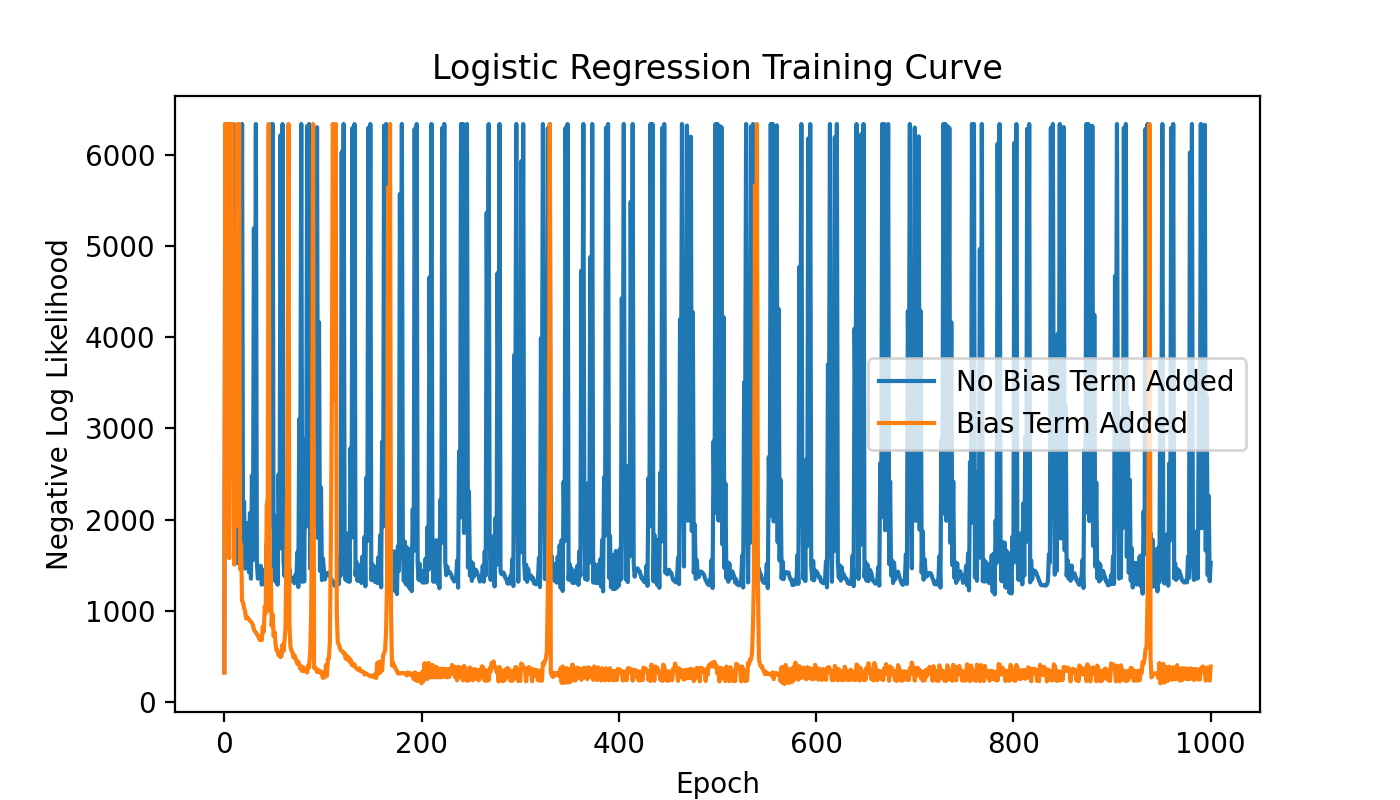
\includegraphics[scale=0.75]{figures/step_size_0.1.png}
\end{mdframed}
\begin{mdframed}[]
    \fbox{$n = 0.01$}
    \begin{verbatim}
Running cross-fold validation for bias case:
2-fold Cross Val Accuracy -- Mean (stdev): 93.78% (1.931%)
3-fold Cross Val Accuracy -- Mean (stdev): 93.76% (2.531%)
4-fold Cross Val Accuracy -- Mean (stdev): 96.36% (2.121%)
5-fold Cross Val Accuracy -- Mean (stdev): 95.67% (2.892%)
10-fold Cross Val Accuracy -- Mean (stdev): 96.3% (3.004%)
20-fold Cross Val Accuracy -- Mean (stdev): 95.42% (4.732%)
50-fold Cross Val Accuracy -- Mean (stdev): 96.38% (5.988%)
    \end{verbatim}
    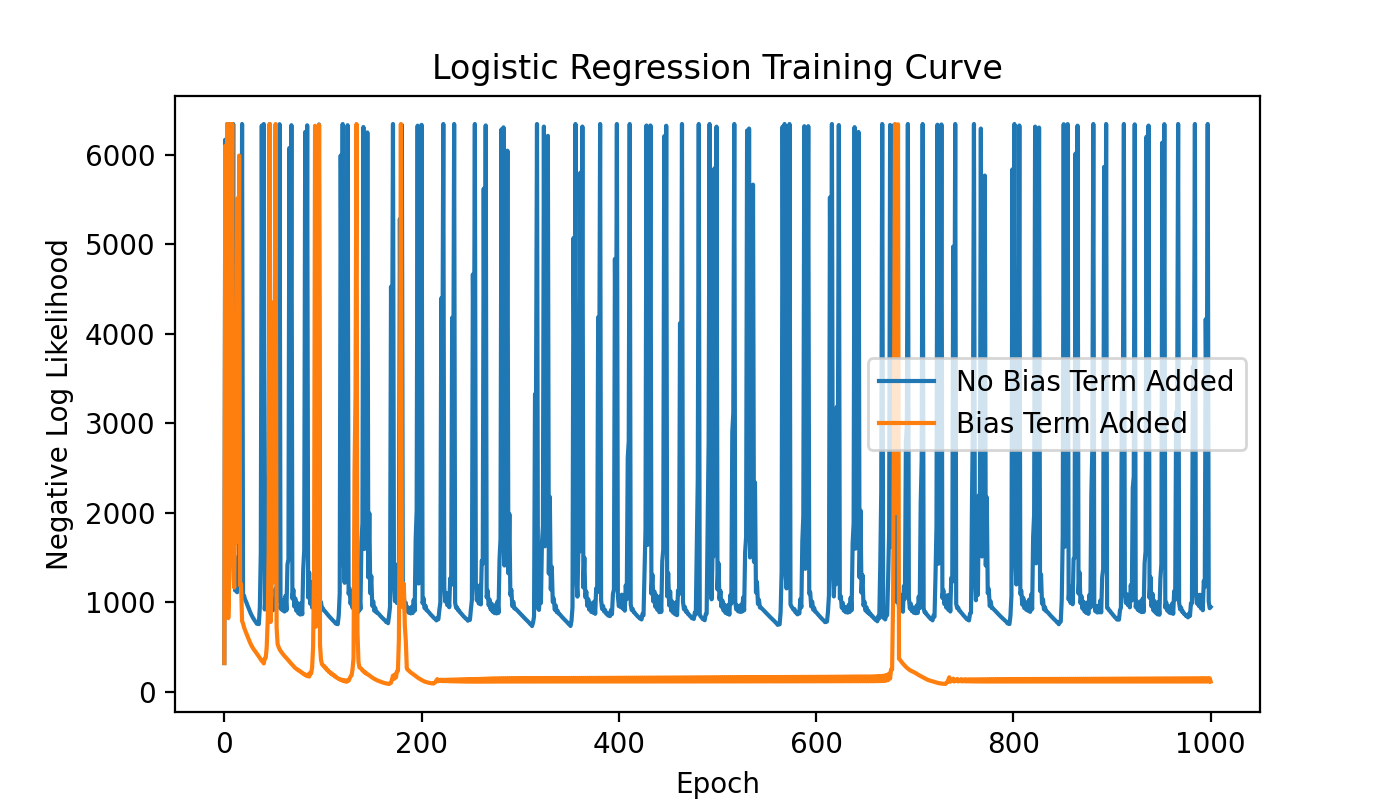
\includegraphics[scale=0.75]{figures/step_size_0.01.png}
\end{mdframed}
\begin{mdframed}[]
    \fbox{$n = 0.0001$}
    \begin{verbatim}
Running cross-fold validation for bias case:
2-fold Cross Val Accuracy -- Mean (stdev): 93.56% (1.717%)
3-fold Cross Val Accuracy -- Mean (stdev): 95.06% (1.349%)
4-fold Cross Val Accuracy -- Mean (stdev): 95.5% (1.632%)
5-fold Cross Val Accuracy -- Mean (stdev): 95.25% (1.708%)
10-fold Cross Val Accuracy -- Mean (stdev): 95.65% (3.622%)
20-fold Cross Val Accuracy -- Mean (stdev): 95.42% (5.878%)
50-fold Cross Val Accuracy -- Mean (stdev): 95.6% (6.635%)
    \end{verbatim}
    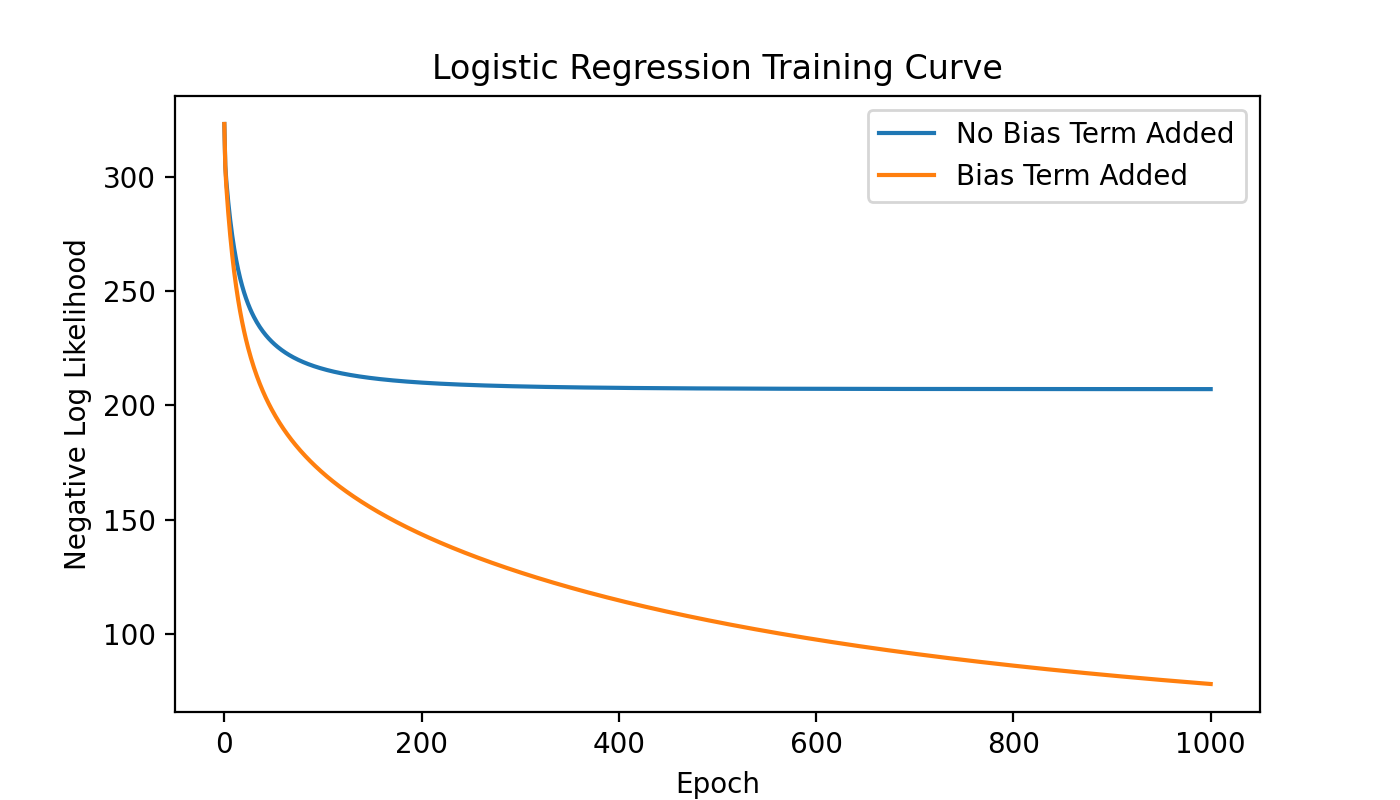
\includegraphics[scale=0.75]{figures/step_size_0.0001.png}
\end{mdframed}
\begin{mdframed}[]
    \fbox{$n = 0.00001$}
    \begin{verbatim}
Running cross-fold validation for bias case:
2-fold Cross Val Accuracy -- Mean (stdev): 87.55% (0.4292%)
3-fold Cross Val Accuracy -- Mean (stdev): 89.26% (2.613%)
4-fold Cross Val Accuracy -- Mean (stdev): 89.71% (1.974%)
5-fold Cross Val Accuracy -- Mean (stdev): 89.93% (3.148%)
10-fold Cross Val Accuracy -- Mean (stdev): 89.9% (3.052%)
20-fold Cross Val Accuracy -- Mean (stdev): 90.42% (8.65%)
50-fold Cross Val Accuracy -- Mean (stdev): 90.35% (9.384%)
    \end{verbatim}
    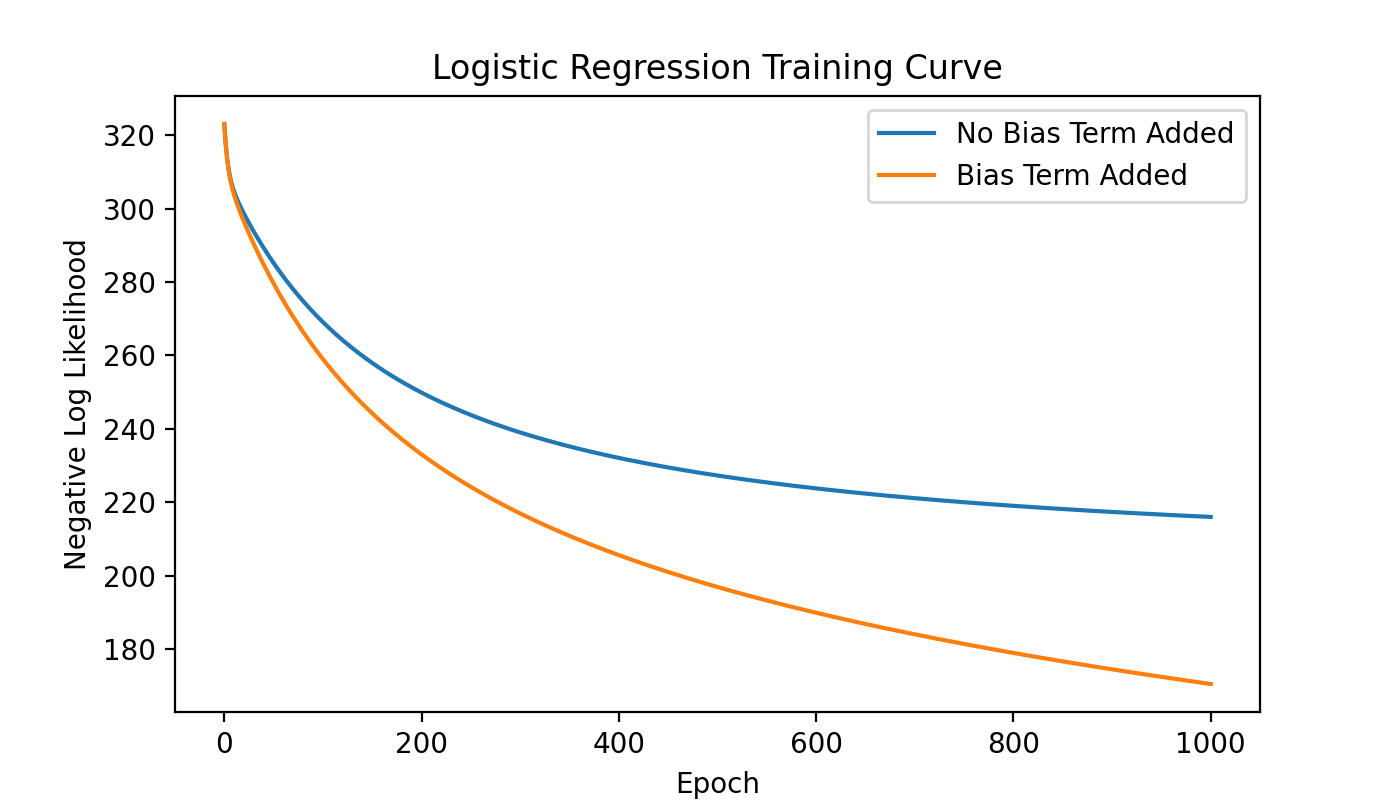
\includegraphics[scale=0.75]{figures/step_size_0.00001.png}
\end{mdframed}
From what we see here, a step size in the order of magnitude around $10^{-4}$ seems to
be about correct for the desired process. It is numerically stable, and it appears that 
it will converge to some actual value much more quickly than something smaller.
For these reasons we think that this will be a good candidate for step size.
    \subsection*{Q7}
Our step size of $n = 0.0001$ had the smallest standard deviations, and the 
highest accuracies, so we concluded that this would be in fact our best candidate for 
the step-size hyperparameter. Using this parameter for our Kaggle submission, in 
combination with a normalization of our data, we see that this was fairly successful and 
resulted in a good score. So, our cross-validation corresponds to a good score in the competition,
so we assume that this a valid and effective metric for hyperparameter searching.
    \subsection*{Q8}
In my final submission I used a step size of $n = 0.0001$ and a max iterations of $i = 10000$. 
I also normalized the data from a 1-10 scale to a 0-1 scale.
\section*{Section 3}
Debriefing:
\begin{verbatim}
1.) Spend about 12 hours on this assignment.
2.) I would rate this as difficult.
3.) I worked on this one mostly alone, but did help my friend debug some 
    issues that he was having.
4.) I feel that I understand the material about 30%.
5.) No other comments.
\end{verbatim}
\end{document}